\documentclass[12pt]{article}
%--------------------   start of the 'preamble'
%
\usepackage{graphicx,amssymb,amstext,amsmath,color}
\usepackage{grffile}
\usepackage[margin=2cm]{geometry}
\usepackage{abstract}
\usepackage{setspace}
\usepackage[footnotesize,bf]{caption}

% TABLE
\usepackage{multicol,hhline,colortbl,multirow}
\usepackage{adjustbox}
\usepackage{braket}
\usepackage{siunitx}
\usepackage{hyperref}
\usepackage{authblk}
\usepackage{siunitx}
\usepackage{mathrsfs}
%%\usepackage[sort&compress]{natbib}
%%\bibpunct{(}{)}{,}{a}{, }{;}
%
\usepackage[sort&compress]{natbib}
\bibpunct{[}{]}{,}{s}{}{;}


\definecolor{gray}{gray}{0.8}
\def\mobunits{\square\centi\meter\per\volt\per\second}
\def\gcm{\gram\per\cubic\centi\meter}
\def\ccg{\cellcolor{gray}}

\renewcommand{\labelitemii}{$\circ$}
\renewcommand{\bibname}{References}


\title{MorphCT - P3HT Paths and Mobility With Fixed Hopping Rates}
\author{Matthew Jones}
\date{\today}

\begin{document}
\maketitle


\section{Motivation}


We are trying to see if Olga's tortuosity calculations can help predict the P3HT mobilities without having to perform the expensive quantum chemical calculations.
To assist with this, we constrain the intra- and inter-molecular hopping rates to be fixed to the average hopping rates calculated through ZINDO/S for a) each of the five P3HT statepoints, and b) the global average over all 5 statepoints.


\textcolor{red}{These jobs are still running but have generated reliable values.
I will update the numbers when the jobs complete, but I would not expect the values to change significantly, nor would I expect the trends to change.}


\section{Summary}

\subsection{Per-Statepoint Average}

The mobility trends are approximately the same when the average hopping rate is taken, as expected.
The absolute value of the mobility has increased by an order of magnitude.
This is likely because all inter-molecular hops have been set to the average rate of the hops taken in the KMC, rather than the average of all available hops.
Previous hops that might have had a rate of 1E12 (because, for instance, the chromophores were so far apart) are now 2 orders of magnitude more likely to happen, resulting in a larger number of longer-range hops and a higher mobility.


\subsection{Global Average}


When all systems are given the same global average rates, the mobility trend is reversed.
This suggests that the pathways through the morphology are somehow better in a disordered morphology than an ordered one.
I wonder if this might be a function of the density.
Now that all hops are equally likely, mobility is no longer governed by the rate at which hops can occur, but instead the distance travelled for each hop.
The disordered morphologies are significantly less dense than the ordered morphology, and so it stands to reason that the chromophores are generally further apart.
This means that carriers are hopping further in the same amount of time in the disordered morphologies, compared to the ordered one.
\textcolor{red}{Should we repeat this investigation but for the systems that were shrunk down to the correct density to see if the usual trend returns?}
Perhaps another thing of note here is that there is only a factor of two difference between the low ordered morphology mobility and the highest disordered mobility.


\section{Mobility Results}


\begin{center}
    \begin{adjustbox}{max width=\textwidth}
\begin{tabular}{| c | c | c | c | c | c | c | c |}
\hline
\rule{0pt}{2.5ex} 
\multirow{2}{*}{\textbf{ID}}&\multirow{2}{*}{\textbf{Simulation Name}}&\textbf{Density}&\textbf{Anisotropy}&\textbf{Intra-Mol Rate}&\textbf{Inter-Mol Rate}&\textbf{Stacks}&\textbf{Mobility}\\
                            &&(\SI{}{\gcm})&(Arb. U.)&(s$^{-1}$)&(s$^{-1}$)&(Arb. U.)&(\SI{}{\mobunits})\\
\hhline{|========|}
\multicolumn{8}{| c |}{\textbf{Original Results}}\\
\hhline{--------}
\textbf{\ccg1}&\rule{0pt}{2.5ex}{\ccg}P3HT\_T1.5&{\ccg}1.676&{\ccg}0.0676&{\ccg}8.07E14&{\ccg}3.92E14&{\ccg}1&{\ccg}1.17$\times 10^{1}$\\
\textbf{2}&\rule{0pt}{2.5ex}P3HT\_T1.75&1.061&0.0065&5.86E14&1.47E13&19&3.48$\times 10^{-1}$\\
\textbf{\ccg3}&\rule{0pt}{2.5ex}{\ccg}P3HT\_T2.0&{\ccg}0.892&{\ccg}0.0065&{\ccg}4.99E14&{\ccg}5.22E12&{\ccg}1&{\ccg}4.46$\times 10^{-1}$\\
\textbf{4}&\rule{0pt}{2.5ex}P3HT\_T2.25&0.787&0.0044&4.88E14&5.63E12&5&5.52$\times 10^{-1}$\\
\textbf{\ccg5}&\rule{0pt}{2.5ex}{\ccg}P3HT\_T2.5&{\ccg}0.685&{\ccg}0.0041&{\ccg}4.42E14&{\ccg}2.31E12&{\ccg}25&{\ccg}4.03$\times 10^{-1}$\\
\hhline{--------}
\multicolumn{8}{| c |}{\textbf{Using Per-Statepoint Hop Rate Average}}\\
\hhline{--------}
\textbf{\ccg6}&\rule{0pt}{2.5ex}{\ccg}AvHop\_P3HT\_T1.5&{\ccg}1.676&{\ccg}0.1488&{\ccg}8.07E14&{\ccg}3.92E14&{\ccg}1&{\ccg}2.40$\times 10^{2}$\\
\textbf{7}&\rule{0pt}{2.5ex}AvHop\_P3HT\_T1.75&1.061&0.0038&5.86E14&1.47E13&19&2.21$\times 10^{1}$\\
\textbf{\ccg8}&\rule{0pt}{2.5ex}{\ccg}AvHop\_P3HT\_T2.0&{\ccg}0.892&{\ccg}0.0024&{\ccg}4.99E14&{\ccg}5.22E12&{\ccg}1&{\ccg}1.27$\times 10^{1}$\\
\textbf{9}&\rule{0pt}{2.5ex}AvHop\_P3HT\_T2.25&0.787&0.0074&4.88E14&5.63E12&5&1.42$\times 10^{1}$\\
\textbf{\ccg10}&\rule{0pt}{2.5ex}{\ccg}AvHop\_P3HT\_T2.5&{\ccg}0.685&{\ccg}0.0031&{\ccg}4.42E14&{\ccg}2.31E12&{\ccg}25&{\ccg}7.81$\times 10^{0}$\\
\hhline{--------}
\multicolumn{8}{| c |}{\textbf{Using Global Hop Rate Average}}\\
\hhline{--------}
\textbf{\ccg11}&\rule{0pt}{2.5ex}{\ccg}AvHop\_P3HT\_T1.5&{\ccg}1.676&{\ccg}0.0532&{\ccg}3.59E14&{\ccg}8.50E13&{\ccg}1&{\ccg}5.45$\times 10^{1}$\\
\textbf{12}&\rule{0pt}{2.5ex}AvHop\_P3HT\_T1.75&1.061&0.0039&3.59E14&8.50E13&19&7.61$\times 10^{1}$\\
\textbf{\ccg13}&\rule{0pt}{2.5ex}{\ccg}AvHop\_P3HT\_T2.0&{\ccg}0.892&{\ccg}0.0020&{\ccg}3.59E14&{\ccg}8.50E13&{\ccg}1&{\ccg}8.63$\times 10^{1}$\\
\textbf{14}&\rule{0pt}{2.5ex}AvHop\_P3HT\_T2.25&0.787&0.0005&3.59E14&8.50E13&5&9.33$\times 10^{1}$\\
\textbf{\ccg15}&\rule{0pt}{2.5ex}{\ccg}AvHop\_P3HT\_T2.5&{\ccg}0.685&{\ccg}0.0041&{\ccg}3.59E14&{\ccg}8.50E13&{\ccg}25&{\ccg}1.14$\times 10^{2}$\\
\hhline{--------}
\end{tabular}\label{table:mob}
\end{adjustbox}
\captionof{table}{The results from MorphCT.}
\end{center}


\begin{figure}[h]\centering
	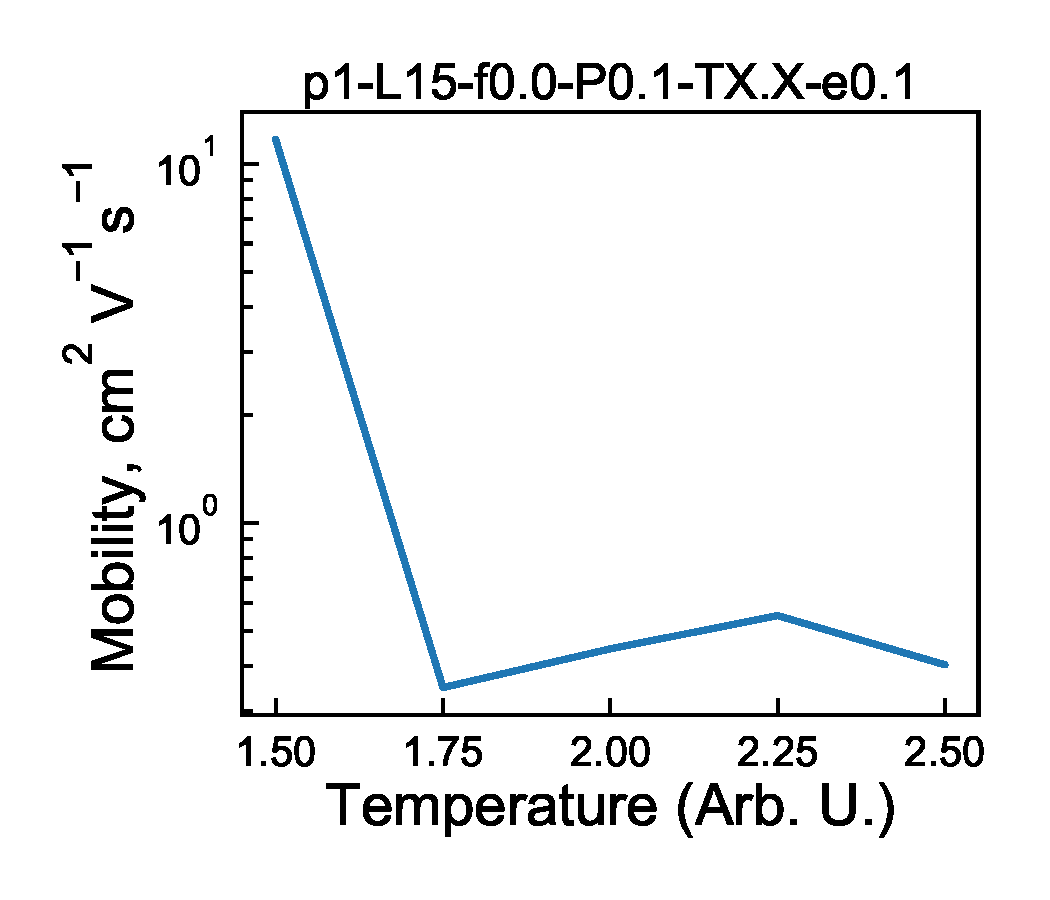
\includegraphics[width=0.5\textwidth]{Figures/mobilityHole.pdf}
    \caption{Original mobility from the P3HT morphologies}
	\label{fig:mobOrig}
\end{figure}


\begin{figure}[h]\centering
	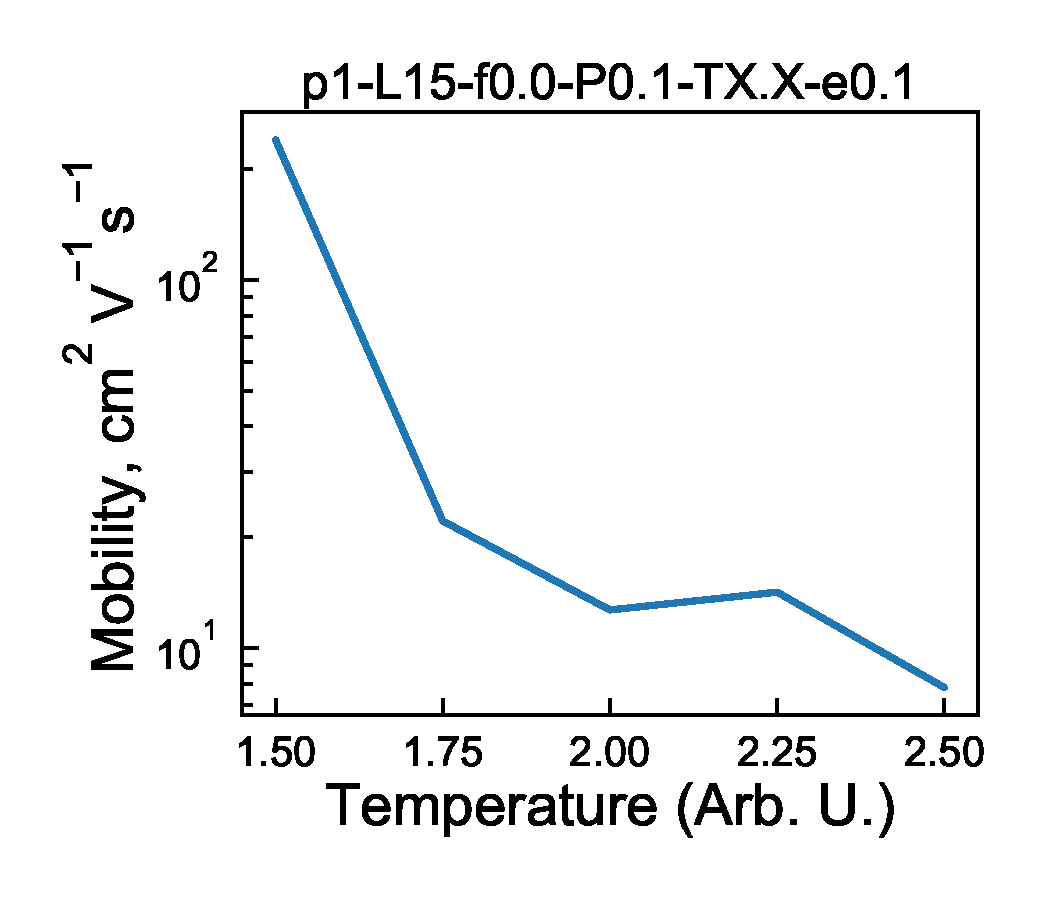
\includegraphics[width=0.5\textwidth]{Figures/2hoursAvHopMobility.pdf}
    \caption{Mobility from the P3HT morphologies, when all hopping rates are fixed to the average intra- or inter-molecular hop rate for the statepoint}
	\label{fig:mobState}
\end{figure}


\begin{figure}[h]\centering
	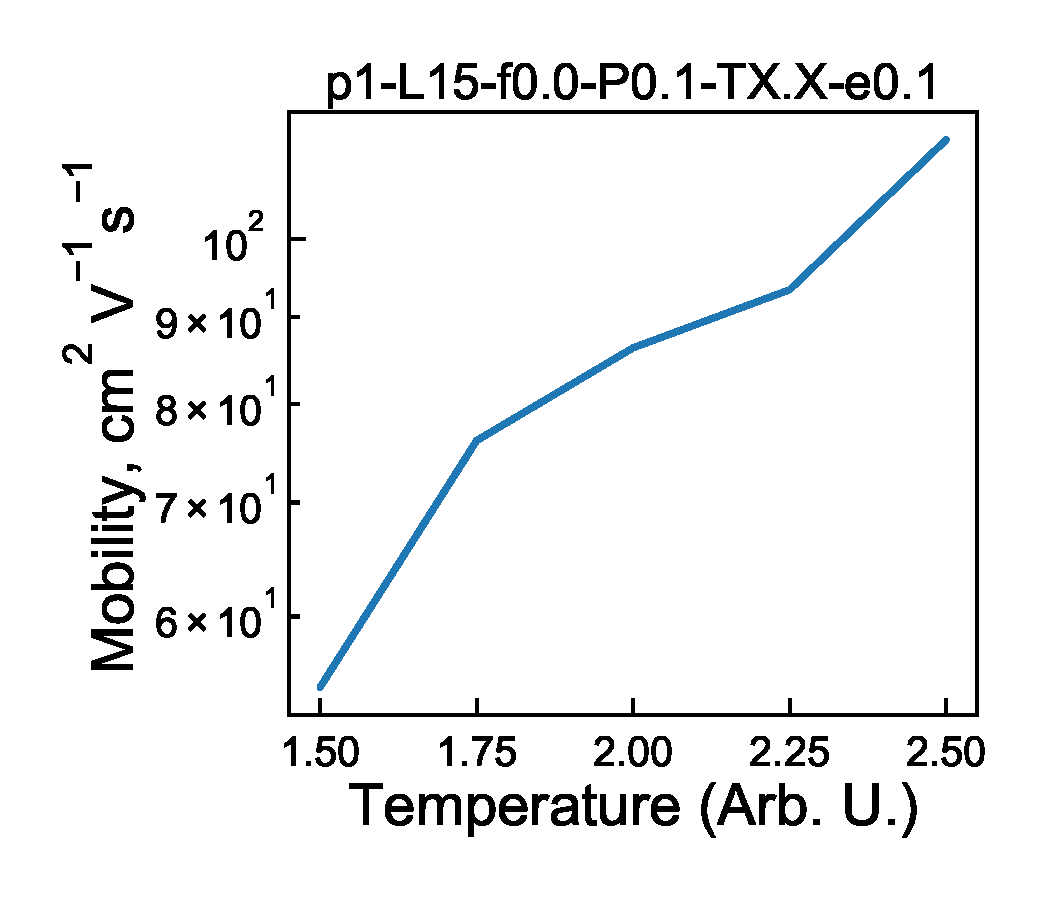
\includegraphics[width=0.5\textwidth]{Figures/2hoursAvHopGlobalMobility.pdf}
    \caption{Mobility from the P3HT morphologies, when all hopping rates are fixed to the average intra- or inter-molecular hop rate for all five statepoints}
	\label{fig:mobGlobal}
\end{figure}


\begin{figure}[h]\centering
	\includegraphics[width=0.85\textwidth]{Figures/avHopP3HT_T1.5.png}
    \caption{   1) Chromophore connectivity network, 
                2) Location of `stacks', 
                3) Distribution of connected chromophore separations (defines stacks),
                4) Density of states of Frontier molecular orbital (delta Eij),
                5) KMC Carrier termination locations (defines anisotropy),
                6) Histogram of molecular transfer integrals,
                7) Histogram of stack transfer integrals,
                8) Histogram of molecular hopping rates,
                9) Histogram of stack hopping rates,
                10) Linear MSD plot,
                11) Semi-log-x MSD plot,
                12) Logarithmic MSD plot.}
	\label{fig:avHopT1.5}
\end{figure}


\begin{figure}[h]\centering
	\includegraphics[width=0.85\textwidth]{Figures/avHopP3HT_T1.75.png}
    \caption{   1) Chromophore connectivity network, 
                2) Location of `stacks', 
                3) Distribution of connected chromophore separations (defines stacks),
                4) Density of states of Frontier molecular orbital (delta Eij),
                5) KMC Carrier termination locations (defines anisotropy),
                6) Histogram of molecular transfer integrals,
                7) Histogram of stack transfer integrals,
                8) Histogram of molecular hopping rates,
                9) Histogram of stack hopping rates,
                10) Linear MSD plot,
                11) Semi-log-x MSD plot,
                12) Logarithmic MSD plot.}
	\label{fig:avHopT1.75}
\end{figure}


\begin{figure}[h]\centering
	\includegraphics[width=0.85\textwidth]{Figures/avHopP3HT_T2.0.png}
    \caption{   1) Chromophore connectivity network, 
                2) Location of `stacks', 
                3) Distribution of connected chromophore separations (defines stacks),
                4) Density of states of Frontier molecular orbital (delta Eij),
                5) KMC Carrier termination locations (defines anisotropy),
                6) Histogram of molecular transfer integrals,
                7) Histogram of stack transfer integrals,
                8) Histogram of molecular hopping rates,
                9) Histogram of stack hopping rates,
                10) Linear MSD plot,
                11) Semi-log-x MSD plot,
                12) Logarithmic MSD plot.}
	\label{fig:avHopT2.0}
\end{figure}


\begin{figure}[h]\centering
	\includegraphics[width=0.85\textwidth]{Figures/avHopP3HT_T2.25.png}
    \caption{   1) Chromophore connectivity network, 
                2) Location of `stacks', 
                3) Distribution of connected chromophore separations (defines stacks),
                4) Density of states of Frontier molecular orbital (delta Eij),
                5) KMC Carrier termination locations (defines anisotropy),
                6) Histogram of molecular transfer integrals,
                7) Histogram of stack transfer integrals,
                8) Histogram of molecular hopping rates,
                9) Histogram of stack hopping rates,
                10) Linear MSD plot,
                11) Semi-log-x MSD plot,
                12) Logarithmic MSD plot.}
	\label{fig:avHopT2.25}
\end{figure}


\begin{figure}[h]\centering
	\includegraphics[width=0.85\textwidth]{Figures/avHopGlobalP3HT_T1.5.png}
    \caption{   1) Chromophore connectivity network, 
                2) Location of `stacks', 
                3) Distribution of connected chromophore separations (defines stacks),
                4) Density of states of Frontier molecular orbital (delta Eij),
                5) KMC Carrier termination locations (defines anisotropy),
                6) Histogram of molecular transfer integrals,
                7) Histogram of stack transfer integrals,
                8) Histogram of molecular hopping rates,
                9) Histogram of stack hopping rates,
                10) Linear MSD plot,
                11) Semi-log-x MSD plot,
                12) Logarithmic MSD plot.}
	\label{fig:avHopGlobalT1.5}
\end{figure}


\begin{figure}[h]\centering
	\includegraphics[width=0.85\textwidth]{Figures/avHopGlobalP3HT_T1.75.png}
    \caption{   1) Chromophore connectivity network, 
                2) Location of `stacks', 
                3) Distribution of connected chromophore separations (defines stacks),
                4) Density of states of Frontier molecular orbital (delta Eij),
                5) KMC Carrier termination locations (defines anisotropy),
                6) Histogram of molecular transfer integrals,
                7) Histogram of stack transfer integrals,
                8) Histogram of molecular hopping rates,
                9) Histogram of stack hopping rates,
                10) Linear MSD plot,
                11) Semi-log-x MSD plot,
                12) Logarithmic MSD plot.}
	\label{fig:avHopGlobalT1.75}
\end{figure}


\begin{figure}[h]\centering
	\includegraphics[width=0.85\textwidth]{Figures/avHopGlobalP3HT_T2.0.png}
    \caption{   1) Chromophore connectivity network, 
                2) Location of `stacks', 
                3) Distribution of connected chromophore separations (defines stacks),
                4) Density of states of Frontier molecular orbital (delta Eij),
                5) KMC Carrier termination locations (defines anisotropy),
                6) Histogram of molecular transfer integrals,
                7) Histogram of stack transfer integrals,
                8) Histogram of molecular hopping rates,
                9) Histogram of stack hopping rates,
                10) Linear MSD plot,
                11) Semi-log-x MSD plot,
                12) Logarithmic MSD plot.}
	\label{fig:avHopGlobalT2.0}
\end{figure}


\begin{figure}[h]\centering
	\includegraphics[width=0.85\textwidth]{Figures/avHopGlobalP3HT_T2.25.png}
    \caption{   1) Chromophore connectivity network, 
                2) Location of `stacks', 
                3) Distribution of connected chromophore separations (defines stacks),
                4) Density of states of Frontier molecular orbital (delta Eij),
                5) KMC Carrier termination locations (defines anisotropy),
                6) Histogram of molecular transfer integrals,
                7) Histogram of stack transfer integrals,
                8) Histogram of molecular hopping rates,
                9) Histogram of stack hopping rates,
                10) Linear MSD plot,
                11) Semi-log-x MSD plot,
                12) Logarithmic MSD plot.}
	\label{fig:avHopGlobalT2.25}
\end{figure}


\begin{figure}[h]\centering
	\includegraphics[width=0.85\textwidth]{Figures/avHopGlobalP3HT_T2.5.png}
    \caption{   1) Chromophore connectivity network, 
                2) Location of `stacks', 
                3) Distribution of connected chromophore separations (defines stacks),
                4) Density of states of Frontier molecular orbital (delta Eij),
                5) KMC Carrier termination locations (defines anisotropy),
                6) Histogram of molecular transfer integrals,
                7) Histogram of stack transfer integrals,
                8) Histogram of molecular hopping rates,
                9) Histogram of stack hopping rates,
                10) Linear MSD plot,
                11) Semi-log-x MSD plot,
                12) Logarithmic MSD plot.}
	\label{fig:avHopGlobalT2.5}
\end{figure}

\bibliography{refs}
\bibliographystyle{unsrt}


\end{document}
